\documentclass{standalone}
\usepackage{tikz}
\usepackage{tikz-qtree}
\usepackage[makeroom]{cancel}
\usetikzlibrary{fit}


\begin{document} 
	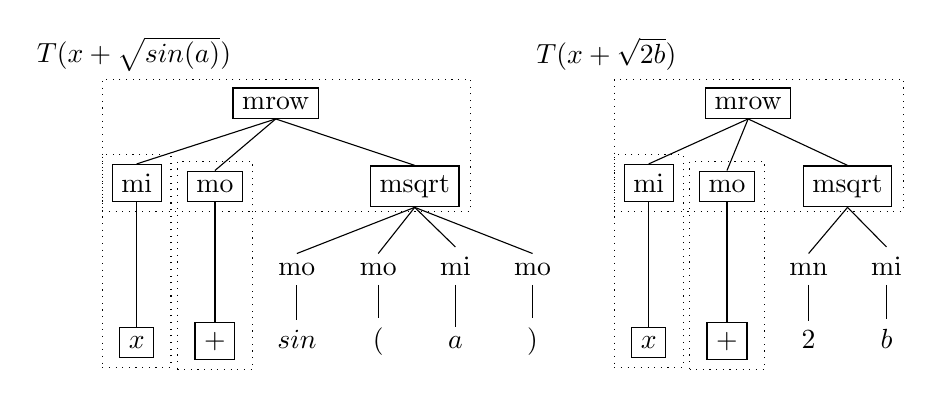
\begin{tikzpicture}[sibling distance=9pt]

		\tikzset{frontier/.style={distance from root=7.2\baselineskip}}
	    \node (x) at (-1.8,0.7) {$T(x + \sqrt{sin(a)})$};
	    \Tree [.\node[draw]{mrow};
	    			[.\node(mi)[draw]{mi}; \node(x)[draw]{$x$}; ]
	    			[.\node(mo)[draw]{mo}; \node(pl)[draw]{$+$}; ]
		            [.\node[draw]{msqrt};
		                [.mo $sin$ ]
		                [.mo $($ ]
		                [.mi $a$ ]
		                [.mo $)$ ] 
		            ] 
	          ]
	    \node (ph) at (2.1,0.02) {\phantom{X}};     
	    \node[draw,dotted,fit=(mi)(x)]{};
	    \node[draw,dotted,fit=(mo)(pl)]{};
	    \node[draw,dotted,fit=(mi)(ph)]{};
	     

	    \begin{scope}[xshift=6.0cm]
		    \node (y) at (-1.8,0.7) {$T(x + \sqrt{2b})$} ;
		    \Tree [.\node[draw]{mrow};
		    			[.\node(mi)[draw]{mi}; \node(x)[draw]{$x$}; ]
		    			[.\node(mo)[draw]{mo}; \node(pl)[draw]{$+$}; ]
			            [.\node[draw]{msqrt};
			            		[.mn $2$ ]
								[.mi $b$ ]
			            ] 
		          ]
		    \node (ph) at (1.6,0.02) {\phantom{X}};
		    \node[draw,dotted,fit=(mi)(x)]{};
		    \node[draw,dotted,fit=(mo)(pl)]{};
		    \node[draw,dotted,fit=(mi)(ph)]{};
	    \end{scope}

	\end{tikzpicture}
\end{document} 